
\documentclass[oneside]{diretrizes}            % Imprimir apenas frente
%\documentclass[doubleside]{diretrizes}        % Imprimir frente e verso

% Importações de pacotes
\usepackage[alf, abnt-emphasize=bf, recuo=0cm, abnt-etal-cite=2, abnt-etal-list=0]{abntex2cite}  % Citações padrão ABNT
\usepackage[utf8]{inputenc}                         % Acentuação direta
\usepackage[T1]{fontenc}                            % Codificação da fonte em 8 bits
\usepackage{graphicx}                               % Inserir figuras
\usepackage{amsfonts, amssymb, amsmath}             % Fonte e símbolos matemáticos
\usepackage{booktabs}                               % Comandos para tabelas
\usepackage{verbatim}                               % Texto é interpretado como escrito no documento
\usepackage{multirow, array}                        % Múltiplas linhas e colunas em tabelas
\usepackage{indentfirst}                            % Endenta o primeiro parágrafo de cada seção.
\usepackage{microtype}                              % Para melhorias de justificação?
\usepackage[algoruled, portuguese]{algorithm2e}     % Escrever algoritmos
\usepackage{float}                                  % Utilizado para criação de floats
\usepackage{times}                                  % Usa a fonte Times
\usepackage{siunitx}

%
% Documento: Preâmbulo
%

\instituicao{Instituto Federal de Educação, Ciência e Tecnologia \\do Rio Grande do Sul}
\abreviatura{IFRS}
\departamento{Campus Restinga}
\local{Porto Alegre}
\programa{Análise e Desenvolvimento de Sistemas}
\nomeautor{Felipe dos Santos Viegas}
\titulotb{Pybot}
%\subtitulo{Subtítulo do trabalho}
\data{2017}
\grau{Tecnólogo}
\dataapresentacao{DD/MM/20AA}

%Dados Orientador
\orientador{Roben Castagna Lunardi}
%\coorientador{Anderson Black}
\instOrientador{IFRS}
\departamentoorientador{Campus Restinga}
\titulacaoorientador{Prof. Me.}

%Dados Coorientador
%\coorientador{Artur Dent}
%\instCoorientador{IFRS}
%\departamentocoorientador{Campus Restinga}
%\titulacaocoorientador{Prof. Dr.}

%Dados Examinador 1
\nmexamum{Mestre dos Magos}
\instexamum{IFRS}
\departamentoexamum{Campus Restinga}
\titulacaoexamum{Prof.}

%Dados Examinador 2
\nomeexamdois{Mestre Splinter}
\instexamdois{IFRS}
\departamentoexamdois{Campus Restinga}
\titulacaoexamdois{Prof. Me.}


% Define as cores dos links e informações do PDF
\makeatletter
\hypersetup{
    portuguese,
    colorlinks,
    linkcolor=black,
    citecolor=black,
    filecolor=black,
    urlcolor=black,
    breaklinks=true,
    pdftitle={Pybot: framework de automação em browser com selenium e python},
    pdfauthor={Felipe Viegas},
    pdfsubject={\imprimirpreambulo},
    hypertexnames=false,
    pdfkeywords={pybot, python, selenium}
}
\makeatother

% Redefinição de labels
\renewcommand{\algorithmautorefname}{Algoritmo}
\def\equationautorefname~#1\null{Equa\c c\~ao~(#1)\null}

% Cria o índice remissivo
\makeindex

% Início do documento
\begin{document}

    % Retira espaço extra obsoleto entre as frases.
    \frenchspacing

    % Elementos pré textuais
    \pretextual
    %
% Documento: Capa
%

\makeatletter
\begin{capa}
	\thispagestyle{empty}%limpa estilo da pagina
	\setlength{\baselineskip}{0.72\baselineskip}
    \begin{center} %Alinhamento centralizado
	

    \textbf{\expandafter\uppercase\expandafter{\imprimirinstituicao}}\\
    \textbf{\expandafter\uppercase\expandafter{\imprimirdepartamento}}\\
    \textbf{\expandafter\uppercase\expandafter{\imprimirprograma}}\\
	\vspace*{5cm}%Espaçamento entre linhas
	\large\textbf{\expandafter\uppercase\expandafter{\imprimirtitulotb}}\\
	\vspace*{6cm}%Espaçamento entre linhas	
	\small\textbf{\expandafter\uppercase\expandafter{\imprimirnomeautor}}\\
	\vspace*{9.5cm}%%Espaçamento entre linhas
	\small\textbf{\expandafter\uppercase\expandafter{\imprimirlocal}}\\
	\small\textbf{\expandafter\uppercase\expandafter{\imprimirdata}}\\
		
		
		
	\end{center} %Alinhamento centralizado
\end{capa}
\makeatother

	

              % Capa
    %
% Documento: FOLHA DE ROSTO
%

\makeatletter
\begin{folhaderosto}
	\thispagestyle{empty}%limpa estilo da pagina
	
    \begin{center}
    
		\small\textbf{\expandafter\uppercase\expandafter{\imprimirnomeautor}}\\
		\vspace*{8.2 cm}%Espaço entre linhas
		\normalsize\textbf{\expandafter\uppercase\expandafter{\imprimirtitulotb}}\\
		
    \end{center}
	
	\vspace*{0.35 cm}%Espaçamento entre linhas
		    \large%tamanho da fonte 
    		\hfill%Estica horizontamente  com espaços
	    	\begin{minipage}{8 cm}%Minipagina
	    		\begin{small} %Muda tamanho da fonte
	    		\setlength{\baselineskip}{0.7\baselineskip}
				
		    	{Trabalho de Conclusão de Curso apresentada como requisito parcial para obtenção do grau de
		    	{\imprimirgrau } em {\imprimirprograma } da {\imprimirinstituicao}{ - }{\imprimirabreviatura},
		    	{\imprimirdepartamento}.}\\{
		    	}\\Orientador: {\imprimirtitulacaoorientador }{ }{\imprimirorientador}\\{
		    	}\\Co-orientador: {\imprimirtitulacaocoorientador }{ }{\imprimircoorientador}
				
				
				\end{small} %Muda tamanho da fonte
		    \end{minipage}%%Minipagina
		    	
		    \vspace*{10 cm}%Espaçamento entre linhas
		    
		    \begin{center} %Alinhamento centralizado
		    	\normalsize %Muda tamanho da fonte
	    		\imprimirlocal\\
	    		\imprimirdata
	    	\end{center}%Alinhamento centralizado

\end{folhaderosto}
\makeatother
        % Folha de rosto
    %
% Documento: FOLHA APROVAÇÃO
%

\makeatletter
\begin{folhadeaprovacao}

\thispagestyle{empty}%limpa estilo da pagina
	
	\begin{center}
    
		\small\textbf{\expandafter\uppercase\expandafter{\imprimirnomeautor}}\\
		\vspace*{3.0 cm}%Espaço entre linhas
		\normalsize\textbf{\expandafter\uppercase\expandafter{\imprimirtitulotb}}
		
    \end{center}
	
	\vspace*{0.35 cm}%Espaçamento entre linhas
		    \large%tamanho da fonte 
    		\hfill%Estica horizontamente  com espaços
	    	\begin{minipage}{8 cm}%Minipagina
	    		\begin{small} %Muda tamanho da fonte
	    		\setlength{\baselineskip}{0.7\baselineskip}
				
		    	{Trabalho de Conclusão de Curso apresentado como requisito parcial para obtenção do grau de
		    	{\imprimirgrau } em {\imprimirprograma } do {\imprimirinstituicao}{ - }{\imprimirabreviatura},
		    	{\imprimirdepartamento}.}\\{
		    	}\\				
				
				\end{small} %Muda tamanho da fonte
		    \end{minipage}%%Minipagina
		    	
		    \vspace*{0.6 cm}%Espaçamento entre linhas
		    
		    \large%%tamanho da fonte 
    		\hfill%%Estica horizontamente  com espaços
	    	 
		    
		    \normalsize %Muda tamanho da fonte
		    \vspace*{1.5 cm}%Espaçamento entre linhas
		    
		    \begin{minipage}{9 cm }%%Minipagina
		    {Data de Aprovação: {\imprimirdataapresentacao}}\\
		    \end{minipage}%Minipagina
			
			\begin{center}%Alinhamento centralizado
		    	\vspace*{1.21 cm}%Espaçamento entre linhas
				\textbf{Banca Examinadora}\\ %Negrito
						
				\vspace*{1 cm}%Espaçamento entre linhas
				\rule{9 cm}{.1 mm}\\
				{\imprimirtitulacaoorientador}{ }{\imprimirorientador} - {\imprimirinstOrientador} - {\imprimirdepartamentoorientador}\\
				Orientador\\
				
				\vspace*{1 cm}%Espaçamento entre linhas
				\rule{9 cm}{.1 mm}\\
				\imprimirtitulacaoexamum{ }\imprimirnmexamum - \imprimirinstexamum - \imprimirdepartamentoexamum\\
				Membro da Banca
				
				\vspace*{1 cm}%Espaçamento entre linhas
				\rule{9 cm}{.1 mm}\\				
								
				\imprimirtitulacaoexamdois{ }\imprimirnomeexamdois - \imprimirinstexamdois - \imprimirdepartamentoexamdois\\
				Membro da Banca
				\vspace*{1.3 cm}%Espaçamento entre linhas
		    \end{center}%Alinhamento centralizado


\end{folhadeaprovacao}
\makeatother
    % Folha de aprovação
    %
% Documento: Folha Catalográfica
%

\thispagestyle{empty}
\vspace*{\fill}

 \begin{flushleft}
\small \setlength{\baselineskip}{0.8\baselineskip}INSTITUTO FEDERAL DE EDUCAÇÃO, CIÊNCIA E TECNOLOGIA DO RIO GRANDE DO SUL\\
Reitor: Prof. Osvaldo Casares Pinto\\
Pró-Reitora de Ensino: Profa. Clarice Monteiro Escott\\
Diretor do Campus Restinga: Prof. Gleison Samuel do Nascimento\\
Coordenador do Curso de Ciência da Computação: Prof. Rafael Pereira Esteves\\
Bibliotecária-Chefe do Campus Restinga: Paula Porto Pedone\\
\end{flushleft}



    %
% Documento: Dedicatória
%

\thispagestyle{empty}
\begin{dedicatoria}

Dedico esse trabalho a todos aqueles que me ajudaram do fim ao começo!

\end{dedicatoria}
       % Dedicatória
    % %
% Documento: Agradecimento
%

\begin{agradecimento}

Neste trecho você faz agradecimentos dirigidos aqueles que contribuíram de maneira relevante a elaboração do trabalho.
Elemento opcional segundo a norma da ABNT NBR 14724 de 2011.

\end{agradecimento}

    % Agradecimentos
    % %
% Documento: Epígrafe
%
\thispagestyle{empty}
\begin{epigrafe}


O fator decisivo para vencer o maior obstáculo é, invariavelmente, ultrapassar o obstáculo anterior.{\\}{\\}

\begin{autorepigrafe}
Henry Ford
\end{autorepigrafe}

\end{epigrafe}


          % Epígrafe
    %
% Documento: Resumo (Português)
%

\begin{RESUMO}
\thispagestyle{empty}
	\begin{SingleSpace}


		Em muitas empresas temos uma certa carência quando o assunto é automação de testes ou processos web em navegadores. A necessidade de testes de regressão, testes de funcionalidades e ou
        automação de processos cresce junto com o sistema, porem a pratica dessas atividades só tem força quando aparece aguma necessidade ou problema.

        Esse novo framework pretende trazer aos usuarios uma ferramenta de facil uso e com recursos uteis para o desenvolvimento dessas tarefas, contando com a facilidade e versatilidade da
        linguagem python e a integração com navegadores com framework selenium.

        O conjuntos de ferarmentas que o framework dispõe são: gerenciamento automatico dos controladores de navegadores(drivers), modulo de relatorios e logs para controle de atividades executadas,
        padronização de criação de elementos de tela utilizando o padrão PageObject.

		\vspace*{0.5cm}\hspace{-1.3 cm}\textbf{Palavras-chave}: Automação, Selenium, Testes.

	\end{SingleSpace}
\end{RESUMO}


          % Resumo na língua vernácula
    %
% Documento: Resumo (Inglês)
%

\begin{ABSTRACT}
	\begin{SingleSpace}


        Currently, many companies lack a solution for  test automation or web process management integrated to the browsers.
        The need for regression testing, functionality testing, and / or process automation grows along with the system,
        but the practice of these activities is only emerge when a need or problem appears.

        In order to solve this problem, we propose a framework aims to present to  users an easy-to-use tool with useful resources for the development of these
        tasks, with the simplicity and versatility of the \textit{Python} language and the integration with browsers with \textit{selenium framework}.

        The sets of tools that the proposed framework presents are: automatic management of the drivers of navigators (\textit{drivers}); module containing reports
        and logs to control activities performed; standardization of screen elements development using the standard \textit{PageObject} and identification of layout change.

		\vspace*{0.5cm}\hspace{-1.3 cm}\textbf{Palavras-chave}: Automation, Selenium, Tests.


	\end{SingleSpace}

\end{ABSTRACT}
          % Resumo em língua estrangeira
    %
% Documento: Lista de figuras
%

\pdfbookmark[0]{\listfigurename}{lof}
\listoffigures*
\cleardoublepage

      % Lista de figuras
    %
% Documento: Lista de tabelas
%

\pdfbookmark[0]{\listtablename}{lot}
\listoftables*
\cleardoublepage
      % Lista de tabelas
    %
% Documento: Lista de abreviaturas e siglas
%

\begin{siglas}
	\setlength{\baselineskip}{0.7\baselineskip}
	
    \item[ABNT] Associação Brasileira de Normas Técnicas
    \item[TCC] Trabalho de Conclusão do Curso
    \item[NBR] Norma Brasileira
\end{siglas}
       % Lista de abreviaturas e siglas
    % %
% Documento: Lista de quadros
%

\pdfbookmark[0]{\listofquadrosname}{loq}
\listofquadros*
\cleardoublepage
      % Lista de quadros
    %%
% Documento: Lista de símbolos
%

\begin{simbolos}
    \item[$ \Gamma $] Letra grega Gama
    \item[$ \lambda $] Comprimento de ondada
    \item[$ \in $] Pertence
\end{simbolos}
     % Lista de símbolos
    \sumario

    % Elementos textuais
    \textual
    %
% Documento: Introdução
%

\chapter{INTRODUÇÃO}\label{chap:introducao}

O ciclo de vida de software tem diveras etapas, de um modo geral elas são: Análise de requisitos, Concepção do Projeto, Desenvolvimento, Implantação e por fim Manutenção.
Nas etapas de Desenvolvimento e a Manutenção é onde a criação ou a codificação do software em questão mais acontece, e na concepção de um projeto a necessidade da criação
de um processo de testes que cresça junto do sistema não tem a sua devida importação.


Este Trabalho de Conclusão de Curso tem como objetivo criar um framework para auxiliar nas tarefas de criação de testes e ou automatização de processos de sistemas executados em navegadores.
Levando o nome de PyBot, união das palavras Python, liguagem utilizada para criação do projeto, e Bot, que em inglês quer dizer robô, essa ferramenta propõe prover para os usuarios uma serie
de ferramentas para auxiliar a criação e implantação desses processos, contando uma estrutura de criação dos scripts de teste no padrão PageObject e PageElement, geração de registros de logs
para controle de tarefas e passos executados, verificação de alteração de interfaces e layout dos sites e o gerenciamento automatico de drivers de navegadores com a ferramenta Driloader.            % Introdução
    %
% Documento: Introdução
%

\chapter{TRABALHOS RELACIONADOS}\label{chap:relacionados}

    Conforme \cite{dos2016estudo} a importância da criação de processos automatizados cresce junto da importância que os \emph{softwares} vão tendo na sociedade, e as empresas
    tem uma certa dificuldade quando tentam de adotar ou implantar tais tipos de processos, devido a falta de profissionais com esse conhecimento ou pelas técnicas presentes hoje.

    A solução para automação de testes e processos em navegadores com maior adoção pela comunidade de desenvolvimento de software é o \emph{Selenium} \cite{selenium}.
    O \emph{Selenium} trata-se de uma ferramenta composto por diversos projetos tais como \emph{Selenium Grid}, \emph{Selenium IDE}, \emph{Selenium Remote Control} e o \emph{Selenium WebDriver},
    cada um com suas determinadas funcionalidades. Dentre os projetos citados, o \emph{Selenium WebDriver} é o que mais se assemelha ao projeto proposto pois trata-se de um \emph{framework} para
    integração com navegador, este por sua vez é utilizado como uma das dependências do Pybot(\ref{webdriver}).

    Ainda, outra ferramenta também relacionada ao projeto proposto é o \emph{Robotframework}, esta por sua vez é uma solução bem mais sofisticada, contendo uma quantidade abrangente de módulos
    e usos, porém junto traz uma complexidade maior para seu uso.

    Similar a estes sistemas, a solução proposta neste Trabalho de Conclusão de Curso busca seguir direcionando a integração do \emph{Selenium} com o \emph{Python}. Porém, pretende-se com o Pybot o
    desenvolvimento ferramenta simples e de fácil uso, portanto.

    Para entender melhor o problema, apresenta-se uma análise das funcionalidades e usos das ferramentas citadas anteriormente junto de um comparativo de alguns pontos fortes e
    fracos de cada uma delas.

    \section{Selenium Webdriver}

        \emph{Selenium Webdriver} \cite{webdriver} trata-se de um \emph{framework} onde disponibiliza-se para usuário uma API para integração com o navegador escolhido. Com essa API é possível enviar
        diversos tipos de comandos para o navegador, tais como, verificação e iteração qualquer tipo de elemento presente no DOM (Modelo de Documento Objeto, do inglês \emph{Document Object Model}),
        geração de \emph{prints} de tela e manipulação do próprio navegador, como por exemplo maximizar a janela, redimensionar ou abrir uma nova janela. Todos os comando executados no navegador
        são comandos nativos de cada sistema operacional, sendo necessário possuir o \emph{driver} especifico para cada navegador e sistema operacional para que funcione.

        Ainda, possui suporte as seguintes linguagens de programação: \emph{Java}, \emph{Csharp}, \emph{Python}, \emph{Ruby}, \emph{Php}, \emph{Perl} e \emph{Javascript}. Na maioria
        dos casos, o suporte e funcionalidade são os mesmos para todas linguagens, porém o maior suporte é dado para a linguagem \emph{Java}.


    \section{Robotframework}

        {Robotframework \cite{robotframework} é um dos \emph{frameworks} mais abrangentes disponíveis para teste de software para linguagem \emph{Python}. Esta solução consiste
        de uma vasta variedade de módulos distintos, contando com 11 módulos próprio do \emph{framework} e mais 30 de projetos parceiros, possíveis de serem habilitados. Desta forma,
        possível de optar por incluir determinado módulo ou não no projeto, tendo, também, suporte a \emph{Java} na maioria de seus módulos.

        Sua arquitetura foi feita para executar testes utilizando-se de ATDD (\emph{Acceptance Test Driven Development} ou Desenvolvimento Orientado a Testes de Aceitação) que trata-se de uma
        abordagem ou prática para a criação de requisitos colaborativamente entre o cliente e a equipe e fazendo uso da técnica de desenvolvimento Ágil BDD
        (\emph{Behavior Driven Development} ou Desenvolvimento Guiado por Comportamento em português) onde são criados cenários para cada tipo de comportamento da aplicação é criado levando em
        conta 3 estados, Dado que, Quando e Então, como no exemplo a seguir.

        \vspace*{0,5cm}
        Exemplo: Listas com alguma coisa dentro não podem estar vazias
        \begin{description}
            \item[Dado] que uma nova lista é criada
            \item[Quando] eu adiciono um objeto a ela
            \item[Então] a lista não deve estar vazia.
        \end{description}
        \vspace*{0,5cm}

        O \emph{Robotframework} conta também com os seguinte recursos:
        \begin{itemize}
            \item geração de relatórios de execução, tanto de sucesso como em falhas;
            \item interface por linha de comando;
            \item resposta de execução por XML.
        \end{itemize}


    \section{Comparativo}

    Foram levantados alguns dos pontos mais relevantes para a execução dos \emph{scripts} de testes de cada um dos \emph{framework} e feito uma tabela comparativa entre eles.
    Ambos \emph{frameworks} utilizam em sua base o próprio \emph{framework} \emph{Selenium Webdriver}, portando todas as funcionalidades de integração com os navegadores estarão
    presentes neles e não serão tratadas no comparativo feito a seguir na \autoref{tab:comp}.

    \vspace*{1cm}
\begin{table}[H]
\centering
\caption{Comparativo dos Frameworks}
\label{tab:comp}
\setlength\extrarowheight{7pt}
\begin{tabular}{l|c|c|c}
                                                                                & Selenium                                                                                  & Pybot   & Robotframework \\ \hline
Integração com browser                                                          & Sim                                                                                       & Sim     & Sim            \\ \hline
\begin{tabular}[c]{@{}l@{}}Gerenciamento de drivers\\ dos browser\end{tabular}  & Não                                                                                       & Sim     & Não            \\ \hline
Linguagens Suportadas                                                           & \begin{tabular}[c]{@{}c@{}}Java, C\#, Python, Ruby,\\ Php, Perl e Javascript\end{tabular} & Python  & Python e Java  \\ \hline
\begin{tabular}[c]{@{}l@{}}Supote ao conceito \\ de Page Object\end{tabular}    & Não                                                                                       & Sim     & Sim            \\ \hline
\begin{tabular}[c]{@{}l@{}}Suporte à Técnicas\\ de Desenvolvimento\end{tabular} & Nenhuma                                                                                   & Nenhuma & TDD,BDD e DDT  \\ \hline
Relatorios de Execução                                                          & Nenhum                                                                                    & Erro    & Sucesso e Erro \\ \hline
Arquivo de Configuração                                                         & Não                                                                                       & Sim     & Sim            \\ \hline
Modular                                                                         & Não                                                                                       & Não     & Sim            \\ \hline
Código Aberto                                                                   & Sim                                                                                       & Sim     & Sim
\end{tabular}
\end{table}

\vspace*{-0,9cm}
{\raggedright \fonte{Felipe Viegas, 2017.}}
\vspace*{1cm}



    Como podemos ver, o diferencial é nas funcionalidades especificas de cada um, onde podemos perceber uma separação de níveis. Onde temos uma ferramenta super completa com módulos independentes
    e específicos para cada necessidade dando uma versatilidade maior para usuário em questão de funcionalidades, que é o caso do \emph{Robotframework}, e por outro lado temos outros 2 \emph{frameworks}
    mais básicos, onde o \emph{Pybot} traz melhoria em relação ao \emph{Selenium} padrão, dando uma maior facilidade para os usuários no inicio das tarefas utilizando algumas técnicas para agilizar e organizar
    o desenvolvimento dos \emph{scripts}, relatórios de execução, arquivo de configurações para execução dos \emph{scripts} e controle automático dos \emph{drivers} de cada navegador.


          % Trabalhos Relacionados
    %
% Documento: FRAMEWORK PROPOSTO
%
\chapter{ARQUITETURA DO PYBOT}\label{chap:imp}
    O \textit{framework} proposto foi formado por 4 módulos básicos, cada um com suas devidas utilidades e funções.
    A separação de cada módulo foi criada com base em suas características e funcionalidades, onde temos um modulo responsável pela gerenciamento e
    funcionamento do \textit{framework}, outro pela abstração das páginas dos sistemas \textit{web} a serem mapeados, controle e criação de relatórios
    e logs de execuções e por fim um responsável pelo download e gerenciamento dos \textit{drivers} de cada navegador utilizados pelos \textit{scripts}
    escritos pelos usuários.

    Na Figura \ref{fig:modules} é apresentado um diagrama dos módulos junto das suas classes principais que compõe o
    \textit{framework} e nas próximas seções serão descritas as suas funcionalidades e usos.


    \begin{figure}[H]
        \vspace*{0,3cm}
        \centering
        \caption{Diagrama de Componentes}
        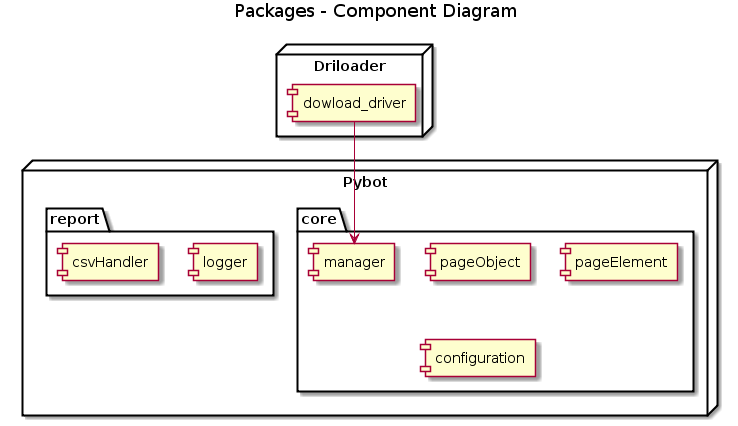
\includegraphics[width=1\textwidth]{./04-figuras/model}
        \label{fig:modules}
    \end{figure}

    \section{Core}
        Este é o módulo principal do framework, nele contém as funcionalidades básicas para a operação do \textit{framework} com o Selenium \textit{Webdriver},
        execução e o gerenciamento dos parâmetros de execuções de cada \textit{script}.

        \subsection{Manager} \label{sec:manager}
        A classe \textit{Manager} é a classe principal do framework, ela serve para abstrair o uso do Selenium \textit{Webdriver} criando uma camada
        de métodos próprios fazendo com que os \textit{scripts} criados com o \textit{Pybot} não sejam impactados por possíveis atualização na API do \textit{Selenium}.
        Dentro dele é feito o uso do \textit{Driloader}, descrito na subseção \ref{driloader} mais a frente, que verifica a necessidade do download do \textit{driver}
        para poder executar o \textit{Selenium Webdriver} e assim abrir o navegador escolhido pelo usuário.

        Como exemplo na Figura~\ref{fig:manager} temos o exemplo de alguns dos comandos disponíveis do Manager, sendo o da linha 4 para o início do processo
        e execução do \textit{driver} do navegador, na linha 7 para navegar para uma URL e na linha 12 para finalizar o processo.

        \begin{figure}[H]
            \vspace*{0,3cm}
            \centering
            \caption{Exemplo - Uso da classe Manager}
            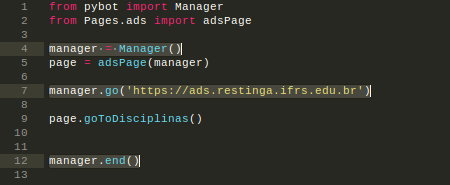
\includegraphics[width=0.8\textwidth]{./04-figuras/manager}
            \label{fig:manager}
        \end{figure}


        \subsection{Configuration}
        Responsável por gerar e gerenciar as configurações básicas para o \textit{framework} e disponibilizá-las no arquivo \textit{pybot.ini} diponivel na mesma pasta que
        o \textit{script}, caso não exista este arquivo é criado automaticamente para cada script. Nele é possível adicionar qualquer configuração ou parâmetros customizado
        do usuário para qualquer necessidade da execução do \textit{script}.

        Na Figura~\ref{fig:config} temos como exemplo apresentado na linha 8 é o código utilizado para buscar uma determinada configuração dentro arquivo \textit{pybot.ini}, sendo ela customizada pelo usuário ou não.

        \begin{figure}[H]
            \vspace*{0,3cm}
            \centering
            \caption{Exemplo - Uso do Configuration}
            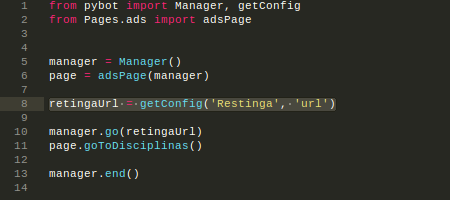
\includegraphics[width=0.8\textwidth]{./04-figuras/config}
            \label{fig:config}
        \end{figure}

        O padrão de escrita das configurações pode ser visto na \autoref{fig:pybot.ini}, onde é necessário ter uma Seção e as variáveis desejadas.
        E para a utilização delas segue o mesmo padrão: \\ \mbox{\textit{configuration.getConfig('Seção', 'variável')}}.

        \begin{figure}[H]
            \vspace*{0,3cm}
            \centering
            \caption{Estrutura pybot.ini}
            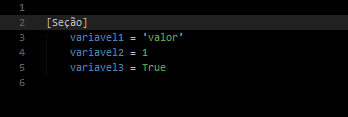
\includegraphics[width=0.7\textwidth]{./04-figuras/ini}
            \label{fig:pybot.ini}
        \end{figure}

        Para o funcionamento correto dos \textit{scripts} o \textit{Pybot} necessita de duas configurações básicas dentro desse arquivo, que são o navegador utilizado na execução e
        o endereço no computador do \textit{driver} desse navegador. Ambas configurações caso não existam são criadas automaticamente.



    \section{Component} \label{sec:comp}
        Módulo criado para seguir os padrões de \textit{PageObject} e \textit{PageElement}, contendo as classes de PageObject e PageElement e a classe responsável
        pela abstração para o \textit{WebElement} do \textit{Selenium Webdriver}.

        Pode-se observar na Figura \ref{fig:eleme} o uso das classes \textit{PageObject}, \textit{PageElement} e \textit{PageElements} nas linhas 3, 4 e 5 respectivamente.

        \begin{figure}[H]
            \vspace*{0,3cm}
            \centering
            \caption{Exemplo - Uso PageObject com PageElement e PageElements}
            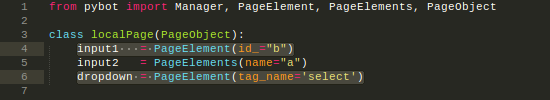
\includegraphics[width=1\textwidth]{./04-figuras/pageElement}
            \label{fig:eleme}
        \end{figure}

        \subsection{PageObject}
            Classe de abstração das páginas web. Serve para poder juntar diversos \textit{PageElement} descritos pelo usuário em uma classe para melhor legibilidade e componentização das
            páginas mapeadas e disponibilizar para os \textit{PageElement} acesso ao navegador.

        \subsection{WebElement}
            Serve para abstrair o uso da classe \textit{WebElement} do próprio \textit{Selenium Webdriver}. Contendo uma classe para cada tipo de campo dos \textit{html},
            ele dispõe de algumas funcionalidades básica, como a atribuição de um valor para um elemento do tipo \textit{input text} irá escrever
            valor dentro do campo, \textit{select} irá selecionar a opção cujo texto seja igual ao valor informado, \textit{radio} irá selecionar o
            a opção que tenha o \textit{value} do valor informado e para o tipo \textit{checkbox} irá marcar ou desmarcar as opções se o valor for
            verdadeiro (\textit{True}) ou falso (\textit{False})

        \subsection{PageElement e PageElements}
        \label{PageElement}
            Essas classes servem para controlar os elementos mapeados das telas. Sempre quando serão acessadas a classe faz novamente a pesquisa
            do elemento em tela, prevenindo assim uma das exceções mais comum do Selenium Webdriver que é a \textit{StaleElementReferenceException},
            que é quando o elemento em questão não existe mais no DOM ou a referência que tinha não é mais a mesma. Conta com uma lista de seletores
            que facilitam para o usuário buscar os elementos e deixam o código mais legível, os mesmos podem ser observados na Figura~\ref{fig:selectors}
            dentro de cada parênteses das definições dos \textit{PageElement}.
            Usa-se a classe PageElements quando quiser pegar mais de um elemento com o mesmo seletor.

            \begin{figure}[H]
                \vspace*{0,3cm}
                \centering
                \caption{Lista de Seletores}
                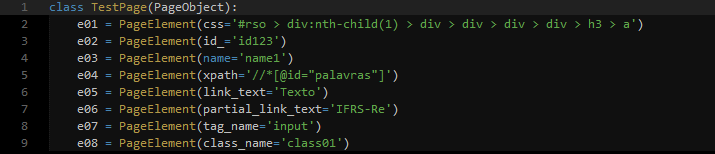
\includegraphics[width=1\textwidth]{./04-figuras/selectors}
                \label{fig:selectors}
            \end{figure}



    \section{Report}

        Este módulo é destinado para geração de \textit{logs} das execuções internas do \textit{framework}, a criação e controle
        de \textit{logs} de execuções de texto e no terminal definidos pelos usuário e a criação de planilhas analíticas de dados extraídos das páginas.

        \subsection{Logger}
        Classe de geração dos \textit{Logs} de execução do \textit{framework}, onde cada execução, ação, sucessos e falhas podem ser configurados para que no
        decorrer do processo sejam mostrados no terminal de execução e no final salvos em um arquivo de texto.

        Os \textit{logs} podem ser configurados com níveis que podem ser \textit{CRITICAL}, \textit{ERROR}, \textit{WARNING}, \textit{INFO} e \textit{DEBUG}, e no arquivo de configurações
        é possível definir qual o nível desejado para que os \textit{logs} apareçam. Numa escala de 1 a 5, \textit{CRITICAL} tem valor 5 e \textit{DEBUG} valor 1, dessa maneira se o nível
        do \textit{log} for definido como \textit{DEBUG} apenas ele aparecerá e se for definido como \textit{CRITICAL} todos apareceram.

        Na \autoref{fig:logs} podemos verificar 2 tipos de escritas do \textit{log}, onde na linha 11 temos a escrita de um \textit{log} e na linha 21 é o tratamento
        de erros de execução, onde este para a execução do código ao ser chamado.

        \begin{figure}[H]
            \vspace*{0,3cm}
            \centering
            \caption{Exemplo - Uso do Logger}
            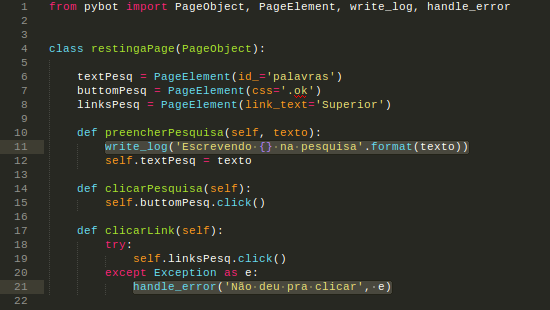
\includegraphics[width=0.9\textwidth]{./04-figuras/logs}
            \label{fig:logs}
        \end{figure}


        \subsection{CsvHandler}
        Utilizado para geração de planilhas com dados extraídos das páginas para análise posterior dos usuários. Os dados têm que ser extraídos manualmente pelo
        usuário, e uma vez extraídos são salvos automaticamente em um arquivo com a extensão \textit{csv}.

        Como exemplo, podemos observar na \autoref{fig:csv} um exemplo de utilização do \textit{CsvHandler}, onde, na linha 5 será criado uma planilha contendo uma
        coluna Disciplina e na linha 21 será inserido registros na planilha abaixo da coluna.

        \begin{figure}[H]
            \vspace*{0,3cm}
            \centering
            \caption{Exemplo - Uso do CsvHandler}
            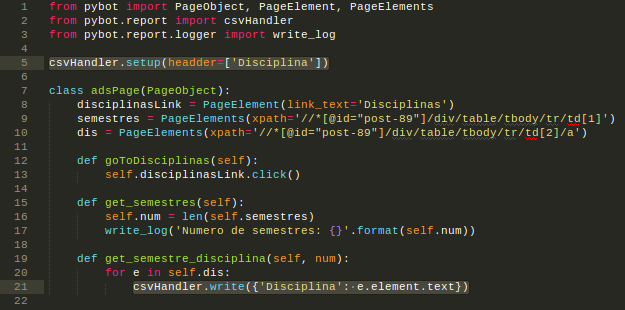
\includegraphics[width=0.9\textwidth]{./04-figuras/csv}
            \label{fig:csv}
        \end{figure}


    \section{Driloader}
    \label{driloader}
        Driloader é o responsável pelo download dos \textit{drivers} de cada navegador, suportando \textit{download} dos \textit{drivers} do \textit{Internet Explorer},
        \textit{Firefox} e \textit{Chrome}, sendo possível para o usuário selecionar uma versão específica, a última versão ou detectar automaticamente qual a versão adequada para o navegador
        instalado do usuário. Como para utilização do \textit{Selenium Webdriver} é necessário um \textit{driver} específico de cada navegador foi tomada a decisão da criação
        desse projeto que inicialmente era um módulo do \textit{framework}, mas pela autonomia e praticidade que ele proporciona aos usuários do Selenium Webdriver foi feita a
        separação dele do \textit{Pybot}. Seu uso é feito na classe Manager (\autoref{sec:manager}) automaticamente quando nenhuma \textit{driver} é encontrado no computador do usuário.



           % Arquitetura
    %
% Documento: Disposições
%

\chapter{TECNOLOGIAS EMPREGADAS}\label{chap:tec}

        Para o desenvolvimento do \textit{framework} foi utilizado apenas como linguagem para desenvolvimento o \textit{Python} na versão \textit{3.6}
        e para a manipulação e integração com o navegador a biblioteca em \textit{Python} do \textit{Selenium Webdriver} tambem na versão \textit{3.6}.
        Por ser um projeto que visa ser o mais simples e leve suas dependências são minimas, fazendo uso apenas dos módulos padrões do \textit{Python}
        e do \textit{Selenium Webdriver} para o desenvolvimento desta ferramenta.

        \section{Python}

            Foi escolhido o \textit{Python} \cite{Python} por que se trata de uma linguagem de programação fácil de aprender e poderosa. Possuindo uma
            estrutura de dados de alto nível e uma abordagem simples, mas eficaz, para a programação orientada a objetos. Contendo uma Sintaxe elegante
            e tipagem dinâmica, juntamente com uma interpretação natural, tornam a linguagem ideal para criação dos \textit{scripts} do Pybot.

        \section{Selenium WebDriver}
        \label{webdriver}

            \textit{Selenium Webdriver} \cite{webdriver} é um \textit{framework} utilizado para se comunicar e enviar comandos para os navegadores em
            conjunto com um controlador específico de cada navegador. Em comparação com seu antecessor, \textit{Selenium RC}, o \textit{Selenium Webdriver}
            não precisa de um \textit{server} para enviar os comandos para o navegador, sendo preciso apenas a utilização desse controlador. Utilizando
            comando nativos do sistema operacional ao invés de comando \textit{javascript}, usados pelo \textit{Selenium RC}, deixam o \textit{Selenium Webdriver}
            uma excelente ferramenta para integração com diversos navegadores.

        \section{Git e GitHub}

            Para o controle de versões e alterações do código fonte do \textit{framework} e \textit{scripts} de exemplo foi utilizado a ferramenta
            \textit{Git} \cite{git} em conjunto com os servidores do \textit{Github} \cite{github} para hospedagem e gerenciamento. Com eles foi possível
            fazer alterações dos códigos fontes em qualquer computador e gerenciar os erros e melhorias do \textit{framework}.
           % Tecnologias Utilizadas
    %
% Documento: Disposições
%

\chapter{Método de Desenvolvimento Proposto}\label{chap:proj}
    O framework proposto é baseado no conceito de PageObject, onde todas as páginas web são tratadas como objetos.
    Ainda, cada componente que seja necessário para automação, um \emph{input}, \emph{span}, etc, é um atributo desse objeto.

    Para melhor exemplificar o uso do conceito de PageObject será utilizado como exemplo um simples login para 2
    usuários, onde será utilizada uma página que possui dois campos de texto, campo de usuário e outro de senha,
    e um botão para submeter o login.

    Primeiro, utilizou-se um exemplo básico de como o \textit{Selenium} propõe o desenvolvimento mostrado na figura
    \ref{fig:selenium_default}. Primeiro é iniciado o \emph{driver} do navegador, navegar para a URL, depois
    são seguidos 3 passos para cada um dos campos de texto, procurar ele, limpar o conteúdo
    (porque não se sabe se ele possui algum texto pré cadastrado) e enviar os caracteres necessário para
    cada campo e por final, procurar e clicar no campo de submeter. Não é uma método muito viável, pois
    no caso temos 2 logins e o \emph{script} deverá ser duplicado para atender ambas necessidades.

    \begin{figure}[H]
        \vspace*{0,3cm}
        \centering
        \caption{Uso padrão Selenium}
        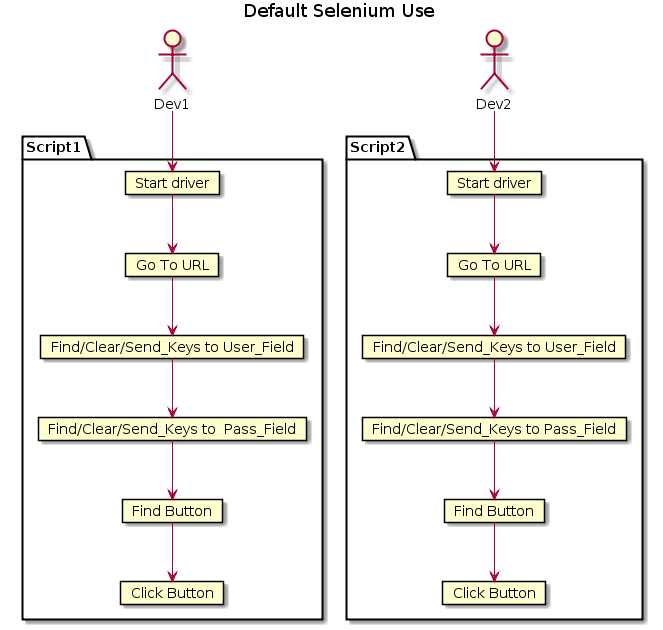
\includegraphics[width=0.8\textwidth]{./04-figuras/page_object_selenium}
        \label{fig:selenium_default}
    \end{figure}

    \clearpage

    Num segundo exemplo poderíamos separar o \emph{script} de login e criar um módulo separado para ele. Desse jeito
    os \emph{scripts} podem fazer uso do mesmo codigo e caso uma terceira pessoa precise dele não seria um problema.
    Porém temos todo o mapeamento dessa página preso num módulo e caso seja necessário a criação de outro
    módulo que use esses campos ainda assim teremos que duplicar mais codigo.

    \begin{figure}[H]
        \vspace*{0,3cm}
        \centering
        \caption{Uso padrão Selenium com módulo}
        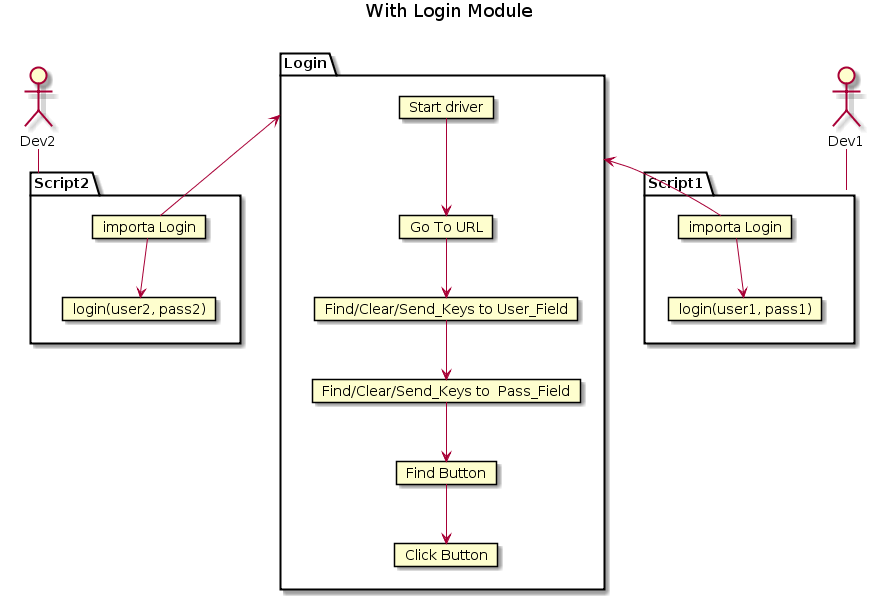
\includegraphics[width=1\textwidth]{./04-figuras/page_object_module}
        \label{fig:selenium_module}
    \end{figure}

    \clearpage
    Chegando num terceiro exemplo onde agora fazemos uso do framework \emph{Pybot}, onde utilizando-se do
    módulo Component(\ref{Comp}) podemos separar todos os componentes da tela em atributos da nossa página
    e criar um método onde precisando de dois parâmetros ele faz o processo de login, e ainda assim, caso
    necessário pode-se utilizar os campos mapeados para fazer algum outro método sem impactar o login.
    E caso alguma referencia dos campos mapeados mude, será necessário alterar apenas um local e nenhum \emph{script}
    será impactado.

    \begin{figure}[H]
        \vspace*{0,3cm}
        \centering
        \caption{Uso padrão Pybot}
        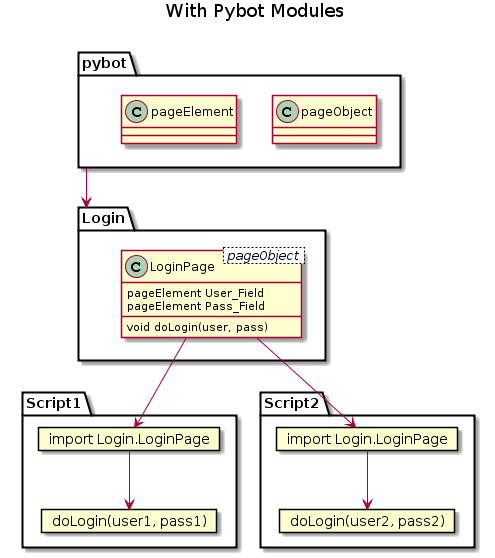
\includegraphics[width=0.8\textwidth]{./04-figuras/page_object_pybot}
        \label{fig:pybot_module}
    \end{figure}               % Uso do projeto
    
\chapter{AVALIAÇÃO DA SOLUÇÃO}\label{chap:result}

    Visando validar se o \textit{framework} proposto atende as necessidades dos usurários foi feito uma pesquisa de uso do \textit{framework} com algumas
    pessoas da área da Programação. Foram executados alguns casos testes e, através da plataforma \textit{Google Forms}, foram aplicadas 5 perguntas
    sobre a experiencia dos usurários com o \textit{framework} em relação ao \textit{Selenium Webdriver}. Num total de 7 usuários foram selecionados
    para criar e executar esses casos de testes e automatiza-los utilizando o \textit{Pybot}, todos os participantes tinham conhecimentos entre básicos
    e intermediário em \textit{Selenium Webdriver} e os cenários foram executados em computadores com \textit{linux} com o \textit{Python} instalado.

    Os casos de testes foram baseados na aplicação web desenvolvida pela empresa em que trabalham e os mesmos eram: criação de \textit{script} de
    \textit{login}, criação de \textit{script} de cadastro e a criação de \textit{script} para extração de dados. Para melhor validação dos \textit{scripts}
    foi pedido para que nos testes fossem utilizados mais de um tipo de seletor para mapeamentos dos campos, iteração com \textit{iframes} e múltiplas
    janelas, geração dos logs de execução e execuções em mais de um browser.

    Com o desenvolvimento e finalização dos \textit{scripts} foram levantados os seguintes pontos sobre a utilização do framework:
    Profissão do Usuário;
    facilidade de instalação;
    facilidade de Uso;
    atende necessidades básicas;
    atende necessidades avançadas.

    A seguir, serão mostrados e analisado os dados coletados em cada um dos pontos do questionário, este que pode ser encontrado nos apêndices deste trabalho.

    \section{Profissão do Usuário}
        Como trata-se de um \textit{framework} de automação de testes foi solicitado um número maior de profissionais da área de \textit{Testes de Software}.
        Como exemplo, pode ser observado na Figura~\ref{fig:profissao}, mais de 70\% dos usuários são Testadores de Software, enquanto menos de 30\% são
        Desenvolvedores.

        \begin{figure}[H]
            \vspace*{0,2cm}
            \centering
            \caption{Profissões}
            \fbox{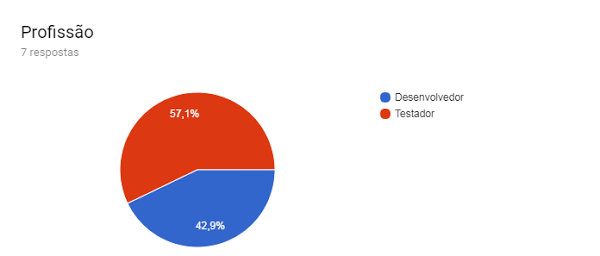
\includegraphics[width=0.8\textwidth]{./04-figuras/profissao}}
            \label{fig:profissao}
        \end{figure}

    \section{Facilidade de instalação}
        Dos usuários na grande maioria consideraram fácil a instalação, como pode ser observado na Figura~\ref{fig:instalacao}. O único ponto a melhorar foi
        que o projeto hoje está disponível apenas pelo repositório do \textit{Github} e não no \textit{PIP}, repositório padrão do \textit{Python}.

        \begin{figure}[H]
            \vspace*{0,2cm}
            \centering
            \caption{Facilidade de instalação}
            \fbox{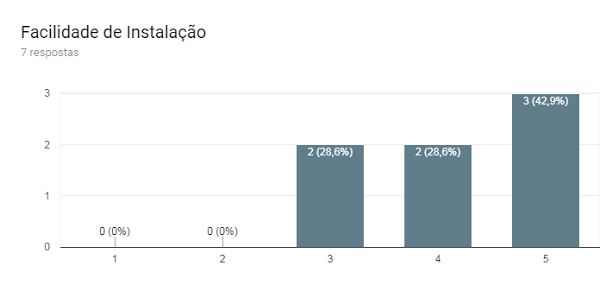
\includegraphics[width=0.8\textwidth]{./04-figuras/instalacao}}
            \label{fig:instalacao}
        \end{figure}

    \section{Facilidade de Usabilidade}

        Em relação a facilidade de uso a grande maioria não teve muitas dificuldades, onde mais de 50\% considerou a usabilidade mediana e o restante de fácil uso,
        como podemos observar na Figura ~\ref{fig:uso}. Onde o maior problema levantado a falta de documentação para verificar todos os comandos de cada classe.

        \begin{figure}[H]
            \vspace*{0,2cm}
            \centering
            \caption{Facilidade de Uso}
            \fbox{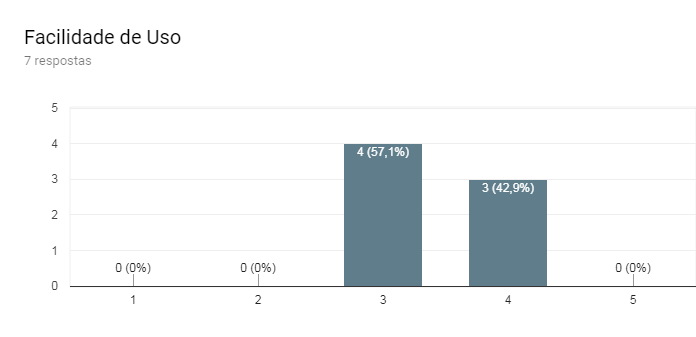
\includegraphics[width=0.8\textwidth]{./04-figuras/uso}}
            \label{fig:uso}
        \end{figure}

    \section{Atende as necessidades básicas}
        As funcionalidades disponíveis do \textit{framework} foram, para a maioria, suficientes para atender as necessidades básicas de criação de um processo de testes.
        Como para a Facilidade de Uso, a documentação também foi um ponto negativo levantado.

          Como pode ser visto na Figura ~\ref{fig:basico}, nenhum usuário classificou com nota 5, o que representa que o \textit{framework} não atende completamente
          todas as necessidades básicas dos usuários.

        \begin{figure}[H]
            \vspace*{0,2cm}
            \centering
            \caption{Atende necessidades básicas}
            \fbox{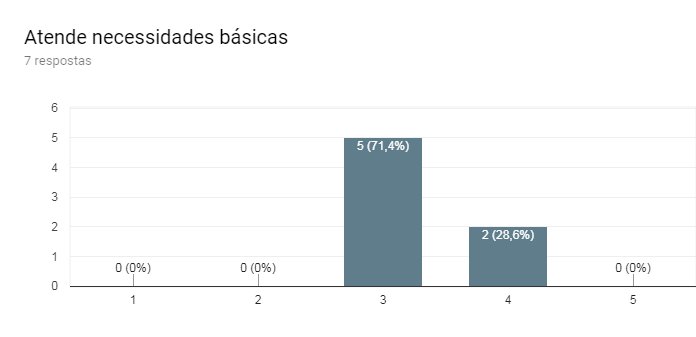
\includegraphics[width=0.8\textwidth]{./04-figuras/basicas}}
            \label{fig:basico}
        \end{figure}

    \section{Atende as necessidades avançadas}
        O \textit{framework} não atingiu as necessidades avançadas. Os usuários tiveram diversos problemas para utilizar múltiplas janelas e elementos renderizados em
        processos assíncronos do \textit{Java\textit{scripts}}, sendo necessário fazer uso do \textit{Selenium} padrão contido no \textit{framework} para realizar tais tarefas.

          Como pode ser visto na Figura~\ref{fig:avancado}, todos os usuários consideraram que o \textit{Pybot} não atendeu necessidades avançadas.

        \begin{figure}[H]
            \vspace*{0,2cm}
            \centering
            \caption{Atende necessidades avançadas}
            \fbox{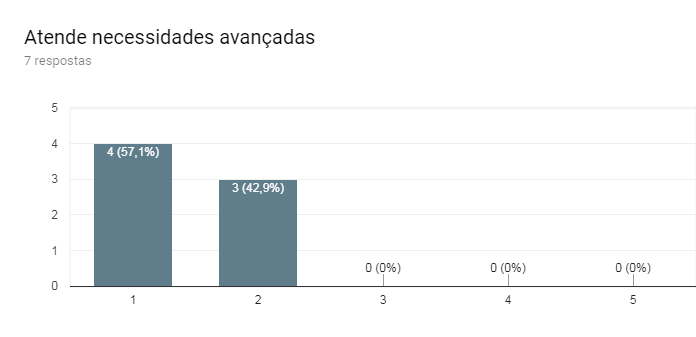
\includegraphics[width=0.8\textwidth]{./04-figuras/avancadas}}
            \label{fig:avancado}
        \end{figure}
               % Analise de dados
    %
% Conclusão
%

\chapter{CONCLUSÃO}\label{chap:conclusao}


    Este trabalho apresentou um \emph{framework} para automatização de testes e processos em navegadores utilizando \emph{Python} e o \emph{framework} \emph{Selenium Webdriver}
    como base, sendo possível a criação de \emph{scripts} de testes em qualquer ambiente sem a necessidade de configurações e instalações complexas.

    Com base nos resultados obtidos pelo questionário aplicado ao usuários no \autoref{chap:result} pode-se observar que o \emph{framework} tem potencial
    para auxiliar os desenvolvedores a criar processos de testes com uma certa facilidade em relação ao \emph{frameworks} existentes atualmente,
    conforme o objetivo do projeto.

    Por fim, com base no desenvolvimento e andamento do projeto foi notado algumas melhorias e trabalhos futuros faltaram para tornar o \emph{Pybot} numa ferramenta
    mais completa, como a criação de uma documentação completa dos módulos, controle de processos assíncronos do \emph{Javascripts}, gerenciamento de múltiplas
    janelas e abas e a hospedagem do \emph{framework} no repositório padrão do \emph{Python}.
             % Conclusão


    % Elementos pós textuais
    \postextual
    %
% Documento: Referências Bibliográficas
%

\bibliography{refbase}    % Geração automática das referências por meio do arquivo 'refbase.bib'
       % Referências
    %
% Documento: Apêndices
%

\begin{apendicesenv}

    \chapter{Pesquisa de satisfação do Pybot}
    \label{app:quest}

    \begin{table}[H]
    \setlength\extrarowheight{25pt}
    \begin{tabular}{lccccc}
        Profissão:                    & (  )         & \multicolumn{1}{l}{Desenvolvedor}  & (  )         & \multicolumn{1}{l}{Testador}   &              \\
        Facilidade de Instalação:     & 1 $\bigcirc$ & 2 $\bigcirc$                       & 3 $\bigcirc$ & 4 $\bigcirc$                   & 5 $\bigcirc$ \\
        Facilidade de Uso:            & 1 $\bigcirc$ & 2 $\bigcirc$                       & 3 $\bigcirc$ & 4 $\bigcirc$                   & 5 $\bigcirc$ \\
        Atende necessidades básicas:  & 1 $\bigcirc$ & 2 $\bigcirc$                       & 3 $\bigcirc$ & 4 $\bigcirc$                   & 5 $\bigcirc$ \\
        Atende necessidades avançadas & 1 $\bigcirc$ & 2 $\bigcirc$                       & 3 $\bigcirc$ & 4 $\bigcirc$                   & 5 $\bigcirc$ \\
        Comentarios:                  & \multicolumn{5}{l}{\_\_\_\_\_\_\_\_\_\_\_\_\_\_\_\_\_\_\_\_\_\_\_\_\_\_\_\_\_}
    \end{tabular}
    \end{table}

    \chapter{Diagramas de Cenários}
    \label{app:imgs}

    \begin{figure}[H]
        \vspace*{0,3cm}
        \centering
        \caption{Uso padrão Selenium}
        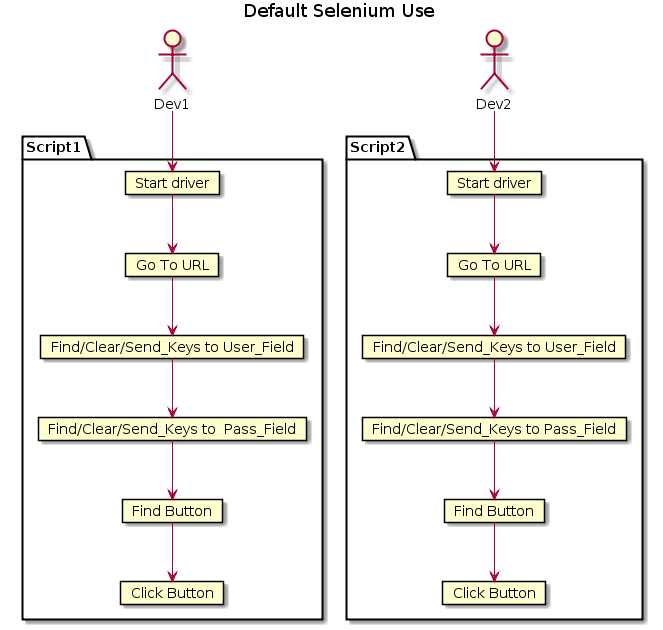
\includegraphics[width=1\textwidth]{./04-figuras/page_object_selenium}
        \label{fig:selenium_default}
    \end{figure}

    \begin{figure}[H]
        \vspace*{0,3cm}
        \centering
        \caption{Uso padrão Selenium com módulo}
        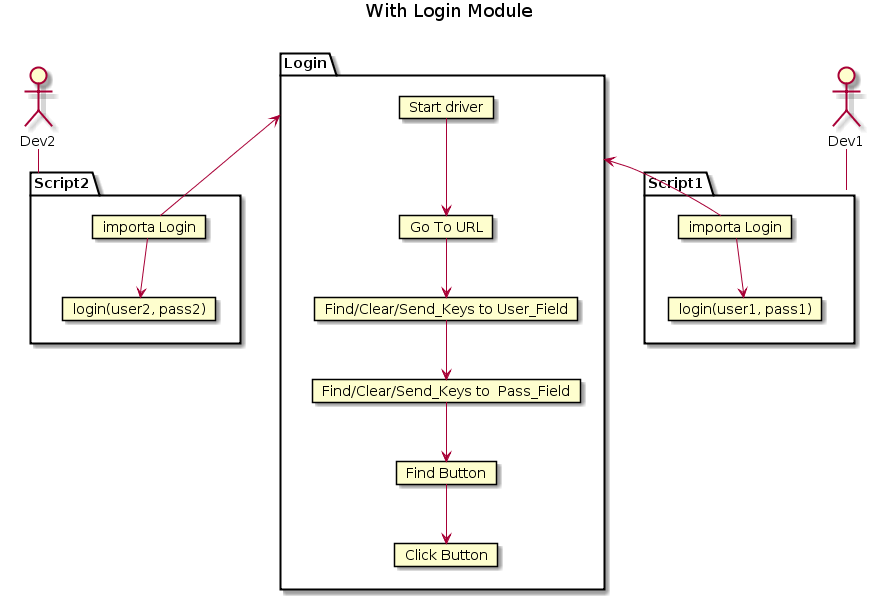
\includegraphics[width=1\textwidth]{./04-figuras/page_object_module}
        \label{fig:selenium_module}
    \end{figure}

    \begin{figure}[H]
        \vspace*{0,3cm}
        \centering
        \caption{Uso padrão Pybot}
        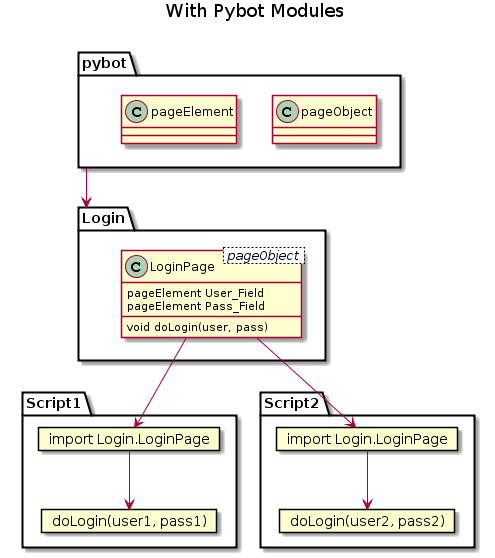
\includegraphics[width=1\textwidth]{./04-figuras/page_object_pybot}
        \label{fig:pybot_module}
    \end{figure}

\end{apendicesenv}         % Apêndices
    %
% Documento: Anexos
%

\begin{anexosenv}

\chapter{Como elaborar}

Anexo é texto ou documento não elaborado pelo autor, que serve de fundamentação, comprovação e ilustração. Elemento opcional. Deve ser precedido da palavra ANEXO, identifi-cado por letras maiúsculas consecutivas, travessão e pelo respectivo título. Utilizam-se letras maiúsculas dobradas, na identificação dos anexos, quando esgotadas as letras do alfabeto.


\end{anexosenv}            % Anexos
    %\printindex                                             % Índice remissivo

\end{document}
